%!TEX root=../../root.tex

\section{Lezione 13}
\subsection{Problemi di decisione}

Un problema può essere visto come l'insieme delle sue istanze, partizionate fra istanze sì e istanze no.
La tesi di Church-Turing afferma che la classe dei linguaggi riconosciuti da una TM corrisponde alla classe dei problemi effettivamente risolvibili. Quindi si può identificare l'idea di algoritmo con quella di una TM che si ferma sempre, mentre un semialgoritmo corrisponde ad una TM che non sempre si ferma.


\subsection{Semi-algoritmo per DFA vuoto}

input: $A = (Q,\Sigma,\delta,q_0,F)$ \\
output: sì se $L(A) \neq \emptyset$ \\
\begin{enumerate}
	\item Poni $x=\varepsilon$
	\item Esegui \emph{A} su \emph{x}
	\item Se \emph{A} accetta \emph{x} rispondi sì
	\item Altrimenti metti in \emph{x} la parola successiva nell'ordine canonico e torna a 2. 
\end{enumerate}

\subsection{Linguaggi non CFL}

\[
	L = \{ \ 0^{2^n} \ | \ n \geq 0 \ \}
\]

\emph{Algoritmo:}
\begin{enumerate}
	\item Sostituisci $B$ con il primo 0 sul nastro
	\item Spostare la testina verso destra sostituendo con \emph{x} ogni secondo 0
	\item Se il nastro non ha altri 0 $\rightarrow$ accetta
	\item Se num(0) è dispari $\rightarrow$ rifiuta
	\item Riporta la testina all'inizio del nastro e torna al punto 2
\end{enumerate}

\begin{figure}[H]
	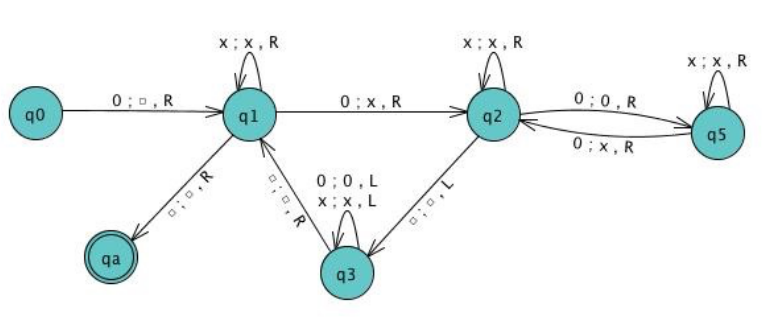
\includegraphics[scale=0.6]{TM1}
\end{figure}


\[
	L = \{ \ a^{n}b^{n}c^{n} \ | \ n \geq 0 \ \}
\]